\documentclass[10pt,twocolumn,letterpaper]{article}

\usepackage{iccv}
\usepackage{times}
\usepackage{epsfig}
\usepackage{graphicx}
\usepackage{amsmath}
\usepackage{amssymb}

% Include other packages here, before hyperref.

% If you comment hyperref and then uncomment it, you should delete
% egpaper.aux before re-running latex.  (Or just hit 'q' on the first latex
% run, let it finish, and you should be clear).
\usepackage[breaklinks=true,bookmarks=false]{hyperref}

\iccvfinalcopy % *** Uncomment this line for the final submission

\def\iccvPaperID{****} % *** Enter the ICCV Paper ID here
\def\httilde{\mbox{\tt\raisebox{-.5ex}{\symbol{126}}}}

% Pages are numbered in submission mode, and unnumbered in camera-ready
%\ificcvfinal\pagestyle{empty}\fi
\setcounter{page}{4321}
\begin{document}

%%%%%%%%% TITLE
\title{What makes an object memorable? }

\author{First Author\\
Institution1\\
Institution1 address\\
{\tt\small firstauthor@i1.org}
% For a paper whose authors are all at the same institution,
% omit the following lines up until the closing ``}''.
% Additional authors and addresses can be added with ``\and'',
% just like the second author.
% To save space, use either the email address or home page, not both
\and
Second Author\\
Institution2\\
First line of institution2 address\\
{\tt\small secondauthor@i2.org}
}

\maketitle
%\thispagestyle{empty}


%%%%%%%%% ABSTRACT
\begin{abstract}
   The ABSTRACT is to be in fully-justified italicized text, at the top
   of the left-hand column, below the author and affiliation
   information. Use the word ``Abstract'' as the title, in 12-point
   Times, boldface type, centered relative to the column, initially
   capitalized. The abstract is to be in 10-point, single-spaced type.
   Leave two blank lines after the Abstract, then begin the main text.
   Look at previous ICCV abstracts to get a feel for style and length.
\end{abstract}

%%%%%%%%% BODY TEXT
\section{Introduction}

Consider the image and it's corresponding objects in Figure \ref{fig:introPhoto}. Even though the person on the right is comparable in size to the left person, he is remembered far less by humans (indicated by their memorability scores of $0.18$ and $0.64$ respectively). People tend to remember the fish in the center and the person on the left, even after $30$ minutes have passed (memorability score $= 0.64$). Interestingly, despite vibrant colors and considerable size, the boat is also remembered far less by humans (memorability $= 0.18$).


\begin{figure}[t]
\centering
\subfigure{\centering 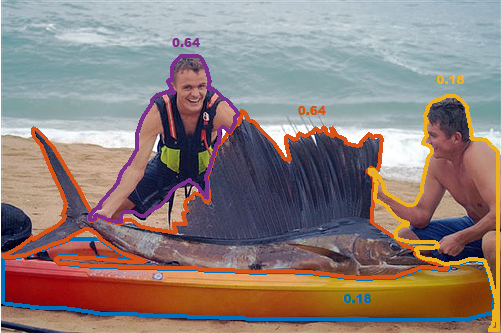
\includegraphics[width=0.2\textwidth]{figures/introduction/intro.png}}
\subfigure{\centering 
\includegraphics[width=0.2\textwidth]{figures/introduction/113.png}}
\vspace{-5mm}\caption{\footnotesize\textbf{Not all objects are equally memorable.} Figure (left) showing how objects in an image have different memorability scores and how this memorability differs from traditional saliency (right). For example, even humans look at the person on the right and find it salient, it's memorability is quite low. }\label{fig:introPhoto}
\end{figure}

Just like aesthetics, interestingness, and other metrics of image importance, memorability quantifies something about the utility of a photograph toward our everyday lives. For many practical tasks, memorability is an especially desirable property to maximize. For example, this may be the case when creating educational materials, logos, advertisements, book covers, websites, and much more. Understanding memorability, and being able to automatically predict it, lends itself to a wide variety of applications in each of these areas.\textcolor{red}{rewrite this to draw attention of reviewer to importance of image memorability}. Due to this, automatic prediction of intrinsic memorability of images using computer vision and machine learning techniques has received considerable attention in the recent years \cite{isola11}, \cite{khosla12}, \cite{isola14}, \cite{zoya15}, \cite{kim13}. While these studies have shed light on what distinguishes the memorability of different images and the intrinsic and extrinsic properties that make those images memorable, the above example raises an interesting question: what exactly about an image is remembered? Despite progress in the computer vision literature on image memorability, a clear understanding of the memorability of the specific components of an image is still unknown. For example, not all objects in an image will be equally remembered by people and as the figure \ref{fig:introPhoto} seems to suggest, there exists significant and interesting differences in memorability of objects in an image. Furthermore, the memorability of complex images may be principally driven by the memorability of it's objects. Can specific objects inside images be memorable to all us and how can we better understand what makes those objects more memorable?

%the memorability of complex images may be principally driven by it's most memorable object, or alternatively, by a combination of particular objects

In this paper, we systematically explore the memorability of objects within individual images and shed light on the various factors and properties that drive object memorability by augmenting both the images and object segmentations in the 850 existing images from PASCAL 2010 \cite{pascal10} dataset with memorability scores and class labels. By exploring the connection between object memorability, saliency, and image memorability, our paper makes several important contributions.

Firstly, we show that just like image memorability, object memorability is a property that is shared across subjects and objects remembered by one person are also likely to be remembered by others and vice versa. Secondly, we show that there exists a strong correlation between visual saliency and object memorability and demonstrate insights when can visual saliency directly predict object memorability and when does it fail to do so. While there have been have a few studies that explore the connection between image memorability and visual saliency \cite{zoya15}, \cite{lemeur13}, our work is the first to explore the connection between object memorability and visual saliency. Third, we explore the connection between image memorability and object memorability and show that the most memorable object inside an image can be a strong predictor of image memorability in certain cases. Studying these questions, help not only understand visual saliency, image and object memorability in more detail, but it can also have important contributions to computer vision. For example, understanding which regions and objects in an image are memorable would enable us to modify the memorability of images which can have applications in advertising, user interface design etc. With this in mind, as shown in the section 4, our proposed dataset serves as a benchmark for evaluating object memorability model algorithms and can help usher in future algorithms that try to predict memorability maps.


\subsection{Related works}

%http://cvcl.mit.edu/papers/IsolaXiaoTorralbaOliva-PredictingImageMemory-CVPR2011.pdf​ ​ In summary, in this paper, a large dataset of images is released wherein the authors ran experiments on human subjects and quantified how memorable each image is. They also ran various analysis on what makes an image more memorable than others. For example, aesthetically pleasing images like landscapes etc are less memorable than an image containing a person. Subsequently, they have showed using computer vision algorithms that they can predict the memorability of images automatically with high accuracy.
%
%http://web.mit.edu/jxiao/Public/publication/2012/NIPSmemorability/paper.pdf​ is a follow up work done by the same authors and is related to memorability of regions in an image i.e. some regions in an image will be more memorable than others. If you go to Figure 4 (pg 7), the authors have built 'memorability maps' for each image via computer vision algorithms. Basically this means that for every pixel (and consequently a region) in an image, their algorithm outputs a memorability value. They then used these memorability maps to predict image memorability from the dataset in the first paper with even greater accuracy. Do note that they have not collected any actual ground truth memorability maps i.e. we still don't know what regions/objects humans consider more memorable in an image.

\textbf{Image Memorability: } Describe Isola's first paper n some insights that have been raised on image memorability thus far. Also describe Khosla's comp model but we are the first work to actually describe what humans actually remember and don't

\textbf{Visual Saliency: } Talk about visual attention and models that have been proposed. Also, talk about Pascal-S and how it has helped reduce dataset bias

\textbf{Saliency and memorability: } discuss some results related to saliency and image memorability. 

and talk about our work plans on connecting and shedding light on all these phenomena together.  
%------------------------------------------------------------------------
\section{Formatting your paper}

All text must be in a two-column format. The total allowable width of the
text area is $6\frac78$ inches (17.5 cm) wide by $8\frac78$ inches (22.54
cm) high. Columns are to be $3\frac14$ inches (8.25 cm) wide, with a
$\frac{5}{16}$ inch (0.8 cm) space between them. The main title (on the
first page) should begin 1.0 inch (2.54 cm) from the top edge of the
page. The second and following pages should begin 1.0 inch (2.54 cm) from
the top edge. On all pages, the bottom margin should be 1-1/8 inches (2.86
cm) from the bottom edge of the page for $8.5 \times 11$-inch paper; for A4
paper, approximately 1-5/8 inches (4.13 cm) from the bottom edge of the
page.

%-------------------------------------------------------------------------
\subsection{Margins and page numbering}

All printed material, including text, illustrations, and charts, must be kept
within a print area 6-7/8 inches (17.5 cm) wide by 8-7/8 inches (22.54 cm)
high.
Page numbers should be in footer with page numbers, centered and .75
inches from the bottom of the page and make it start at the correct page
number rather than the 4321 in the example.  To do this fine the line (around
line 23)
\begin{verbatim}
%\ificcvfinal\pagestyle{empty}\fi
\setcounter{page}{4321}
\end{verbatim}
where the number 4321 is your assigned starting page.

Make sure the first page is numbered by commenting out the first page being
empty on line 46
\begin{verbatim}
%\thispagestyle{empty}
\end{verbatim}


%-------------------------------------------------------------------------
\subsection{Type-style and fonts}

Wherever Times is specified, Times Roman may also be used. If neither is
available on your word processor, please use the font closest in
appearance to Times to which you have access.

MAIN TITLE. Center the title 1-3/8 inches (3.49 cm) from the top edge of
the first page. The title should be in Times 14-point, boldface type.
Capitalize the first letter of nouns, pronouns, verbs, adjectives, and
adverbs; do not capitalize articles, coordinate conjunctions, or
prepositions (unless the title begins with such a word). Leave two blank
lines after the title.

AUTHOR NAME(s) and AFFILIATION(s) are to be centered beneath the title
and printed in Times 12-point, non-boldface type. This information is to
be followed by two blank lines.

The ABSTRACT and MAIN TEXT are to be in a two-column format.

MAIN TEXT. Type main text in 10-point Times, single-spaced. Do NOT use
double-spacing. All paragraphs should be indented 1 pica (approx. 1/6
inch or 0.422 cm). Make sure your text is fully justified---that is,
flush left and flush right. Please do not place any additional blank
lines between paragraphs.

Figure and table captions should be 9-point Roman type as in
Figures~\ref{fig:onecol} and~\ref{fig:short}.  Short captions should be centred.

\noindent Callouts should be 9-point Helvetica, non-boldface type.
Initially capitalize only the first word of section titles and first-,
second-, and third-order headings.

FIRST-ORDER HEADINGS. (For example, {\large \bf 1. Introduction})
should be Times 12-point boldface, initially capitalized, flush left,
with one blank line before, and one blank line after.

SECOND-ORDER HEADINGS. (For example, { \bf 1.1. Database elements})
should be Times 11-point boldface, initially capitalized, flush left,
with one blank line before, and one after. If you require a third-order
heading (we discourage it), use 10-point Times, boldface, initially
capitalized, flush left, preceded by one blank line, followed by a period
and your text on the same line.

%-------------------------------------------------------------------------
\subsection{Footnotes}

Please use footnotes\footnote {This is what a footnote looks like.  It
often distracts the reader from the main flow of the argument.} sparingly.
Indeed, try to avoid footnotes altogether and include necessary peripheral
observations in
the text (within parentheses, if you prefer, as in this sentence).  If you
wish to use a footnote, place it at the bottom of the column on the page on
which it is referenced. Use Times 8-point type, single-spaced.


%-------------------------------------------------------------------------
\subsection{References}

List and number all bibliographical references in 9-point Times,
single-spaced, at the end of your paper. When referenced in the text,
enclose the citation number in square brackets, for
example~\cite{Authors14}.  Where appropriate, include the name(s) of
editors of referenced books.

\begin{table}
\begin{center}
\begin{tabular}{|l|c|}
\hline
Method & Frobnability \\
\hline\hline
Theirs & Frumpy \\
Yours & Frobbly \\
Ours & Makes one's heart Frob\\
\hline
\end{tabular}
\end{center}
\caption{Results.   Ours is better.}
\end{table}

%-------------------------------------------------------------------------
\subsection{Illustrations, graphs, and photographs}

All graphics should be centered.  Please ensure that any point you wish to
make is resolvable in a printed copy of the paper.  Resize fonts in figures
to match the font in the body text, and choose line widths which render
effectively in print.  Many readers (and reviewers), even of an electronic
copy, will choose to print your paper in order to read it.  You cannot
insist that they do otherwise, and therefore must not assume that they can
zoom in to see tiny details on a graphic.

When placing figures in \LaTeX, it's almost always best to use
\verb+\includegraphics+, and to specify the  figure width as a multiple of
the line width as in the example below
{\small\begin{verbatim}
   \usepackage[dvips]{graphicx} ...
   \includegraphics[width=0.8\linewidth]
                   {myfile.eps}
\end{verbatim}
}


%-------------------------------------------------------------------------
\subsection{Color}

Please refer to the author guidelines on the ICCV 2015 web page for a discussion
of the use of color in your document.

%------------------------------------------------------------------------
\section{Final copy}

You must include your signed IEEE copyright release form when you submit
your finished paper. We MUST have this form before your paper can be
published in the proceedings.


{\small
\bibliographystyle{ieee}
\bibliography{egbib}
}

\end{document}
